
\section{Ablation Study}\label{apx:ablation}
In the main paper, we focused on simultaneously replacing both the transition and reward functions with neural networks. This approach allows for greater generality and can be applied across a multitude of environments. However, when only the transition or reward function is differentiable and available, it is feasible to replace only one of them. This simplifies the algorithm, requiring the training of only a single additional network alongside the policy and value functions.

Specifically, we focus on replacing only the reward function. In fact, transition dynamics are often complex and challenging to model with a neural network, especially in multi-agent environments where observations depend not only on the actions of individual agents but also on those of other agents. This, in turn, may necessitate the use of larger architectures with greater computational demands, ultimately limiting the algorithm's practicality.

In contrast, the reward function is often simpler and, therefore, easier to model using lightweight neural networks. Moreover, a high degree of precision is typically not required in most scenarios. As a result, the reward function is an ideal candidate for replacement with a neural network.

This experiment also enables us to compare the final impact of gradients generated by a complex physics engine with those generated by a neural network. While the physics engine may produce more unstable gradients, the neural network may generate imprecise gradients, particularly during the early stages of training.

\subsection{Results}
We refer to the \fname{} algorithm as \fnamer{} when the transition function is differentiable and directly available. The results for the transformer architecture are shown in \Cref{fig:ablation-transformer}, while the results for the MLP architecture are presented in \Cref{fig:ablation-mlp}.

For the transformer architecture, \fname{} generally appears to generate better policies, particularly in the Sampling and Transport environments. In the Dispersion environment, both algorithms perform comparably. Slightly better results are achieved with the \fnamer{} algorithm in the Discovery environment.

For the MLP architecture, the results are more mixed. In the Dispersion environment, \fname{} appears to achieve better policies. Conversely, in the Transport environment, \fnamer{} leads to substantially better policies. In the Discovery environment, both policies struggle to produce meaningful results. Finally, in the Sampling environment, \fname{} performs on par with \fnamer{}, except in the single-agent case, where \fnamer{} struggles.

\subsection{Discussion}
We can easily observe that the transformer architecture leads, generally speaking, to better policies. This is also evident by inspecting \Cref{tab:max-rewards}. This may be due to the positional invariance property of the transformers leading to more sample efficient networks. 

Furthermore, with the transformer architecture, we observe a tendency for \fname{} to produce better results. This may be attributed to the generated gradients being more stable, as shown in \Cref{fig:grads-mlp}.

In contrast, for the MLP architecture, the results are more mixed. This could be attributed to the MLP architecture being less sample-efficient, which ultimately leads to less accurate gradients.

\begin{figure}[t]
    \centering
    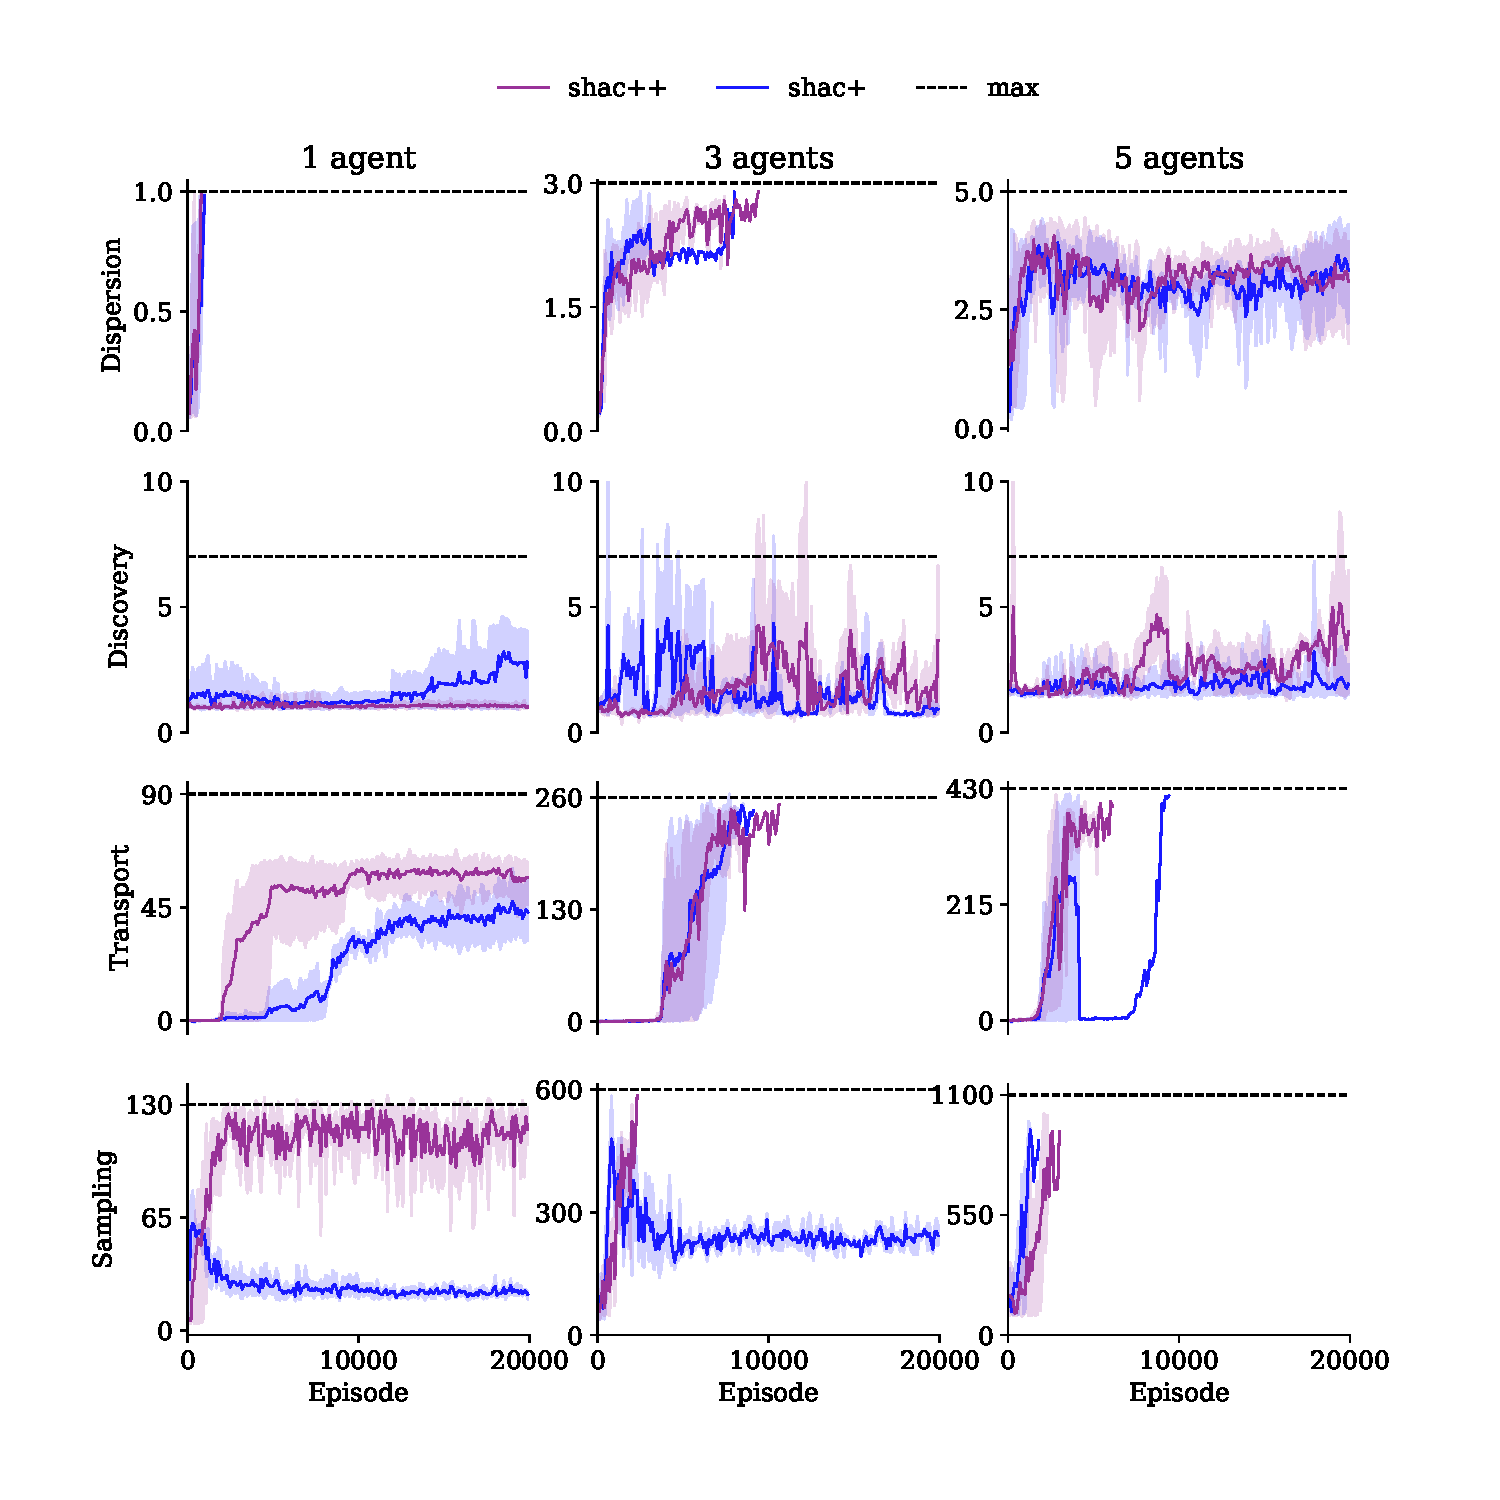
\includegraphics[width=\textwidth]{figs/ablation-transformer.pdf}
    \caption{Comparison between \fname{} with and without transition network, labelled \fnamer{}, for increasing number of agents for Dispersion, Transport, Discovery, and Sampling scenarios. Transformer architecture.}
    \label{fig:ablation-transformer}\vspace{0.5cm}
\end{figure}

\begin{figure}[t]
    \centering
    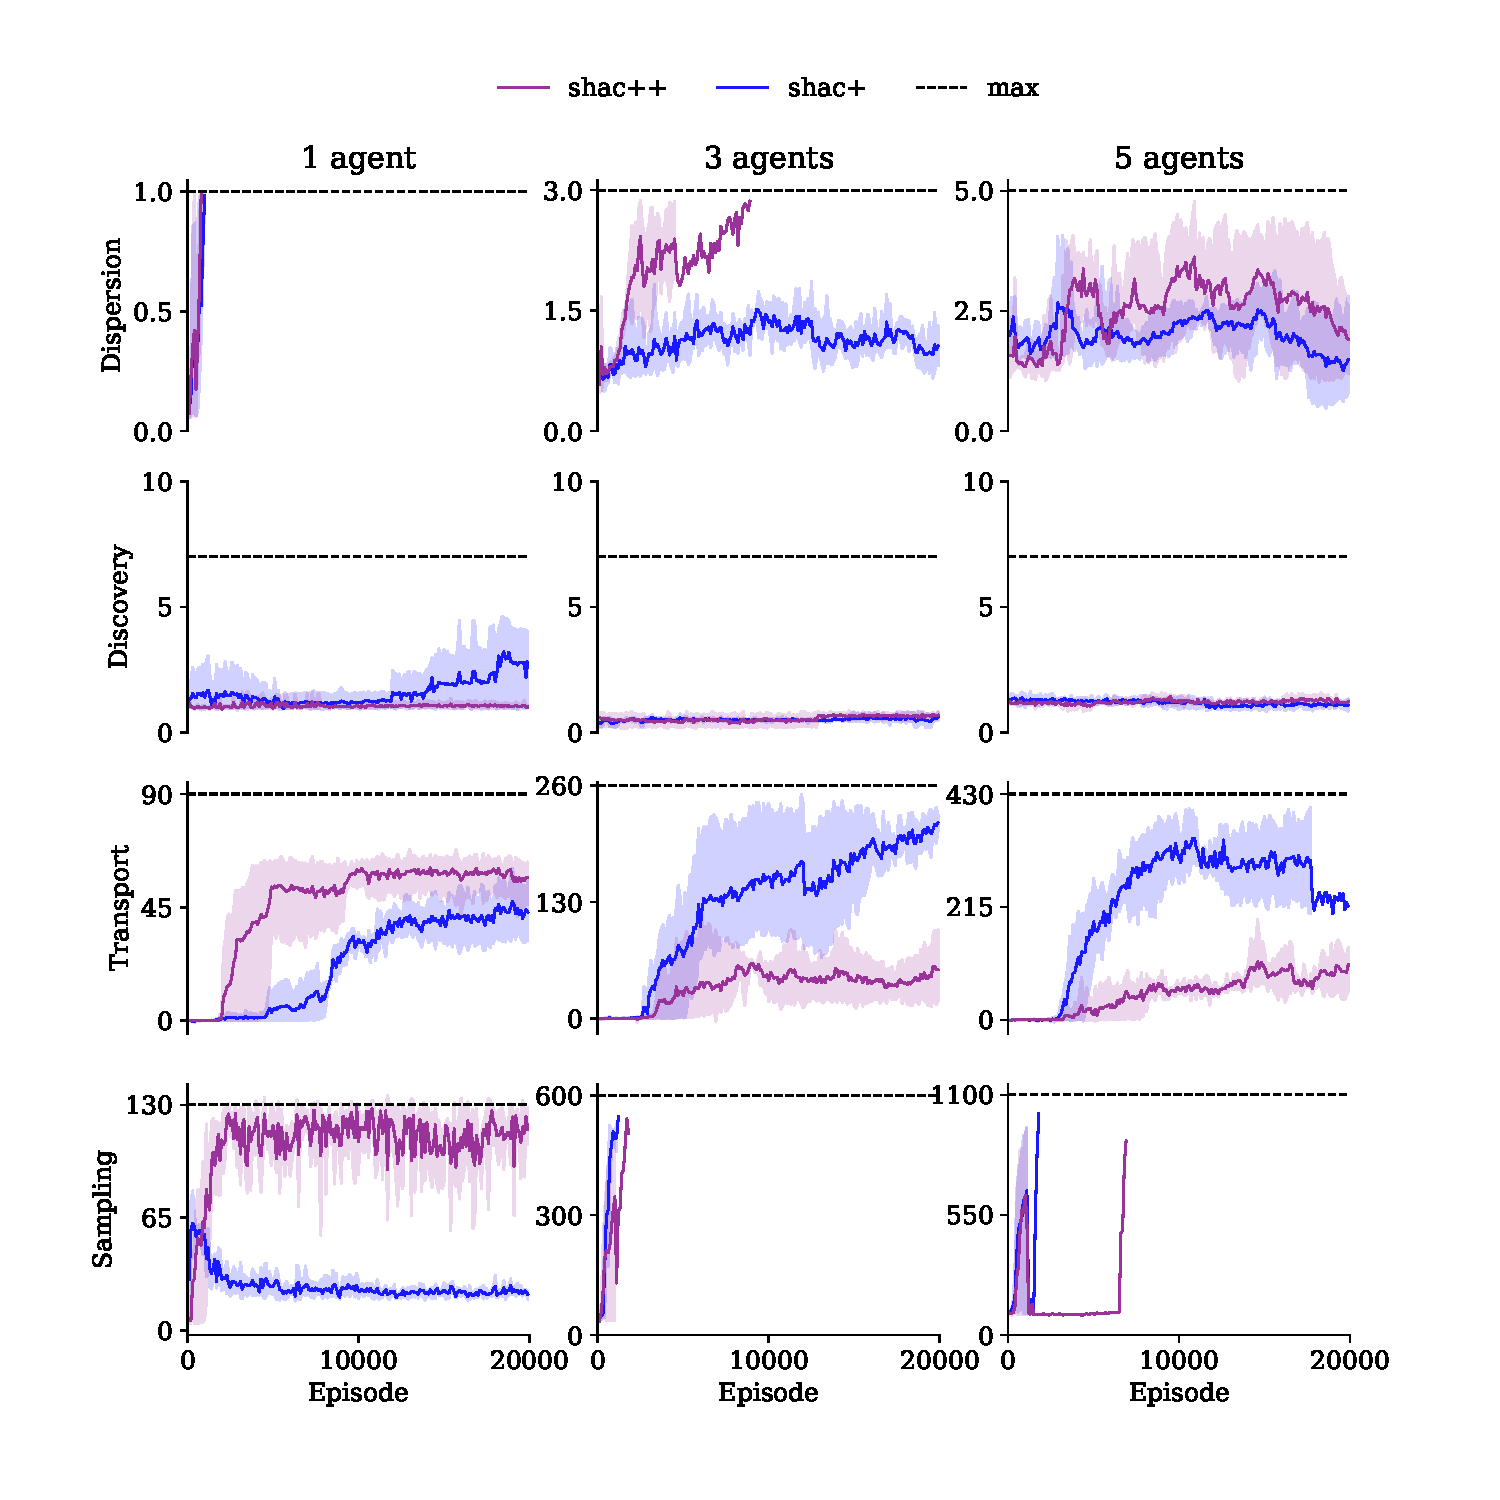
\includegraphics[width=\columnwidth]{figs/ablation-mlp.pdf}
    \caption{Comparison between \fname{} with and without transition network, labelled \fnamer{}, for increasing number of agents for Dispersion, Transport, Discovery, and Sampling scenarios. MLP architecture.}
    \label{fig:ablation-mlp}\vspace{0.5cm}
\end{figure}
\begin{table}[t]
    \begin{minipage}{0.48\textwidth}
        \centering
        \begin{tabular}{ l l l}
	\toprule
	Parameter & Transformer & MLP \\
	\midrule
	number of training environments & 512 & 512 \\
	training horizon & 32 & 32 \\
	number of evaluation environments & 512 & 512 \\
	evaluation horizon & 512 & 512 \\
	policy layers & 1 & 1 \\
	policy hidden size & 64 & {160, 32, 96} \\
	policy feedforward size & 128 & - \\
	policy heads & 1 & - \\
	policy dropout & 0.1 & 0.1 \\
	policy activation & ReLU & ReLU \\
	policy variance & 1 & 1 \\
	value layers & 1 & 1 \\
	value hidden size & 64 & {160, 32, 96} \\
	value feedforward size & 128 & - \\
	value dropout & 0.0 & 0.0 \\
	value activation & ReLU & ReLU \\
	reward layers & 1 & 1 \\
	reward hidden size & 64 & {160, 32, 96} \\
	reward feedforward size & 128 & - \\
	reward dropout & 0.0 & 0.0 \\
	reward activation & ReLU & ReLU \\
	world layers & 3 & 3 \\
	world hidden size & 64 & 64 \\
	world feedforward size & 128 & 128 \\
	world dropout & 0.0 & 0.0 \\
	world activation & ReLU & ReLU \\
	policy learning rate & 0.001 & 0.001 \\
	reward learning rate & 0.001 & 0.001 \\
	value learning rate & 0.001 & 0.001 \\
	value clip coefficient & None & None \\
	reward clip coefficient & None & None \\
	policy clip coefficient & 1 & 1 \\
	world cache size & 30000 & 30000 \\
	reward cache size & 30000 & 30000 \\
	value cache size & 30000 & 30000 \\
	world/value/reward batch size & 1000 & 1000 \\
	world/value/reward cooldown epochs & 10 & 10 \\
	world cache bins & 25 & 25 \\
	reward cache bins & 9 & 9 \\
	value cache bins & 9 & 9 \\
	$\alpha$ & 1.0 & 1.0 \\
	early stopping - max reward fraction & 0.9 & 0.9 \\
	early stopping - max envs fraction & 0.9 & 0.9 \\
	seed & {42, 43, 44} & {42, 43, 44} \\
	max episodes & 20000 & 20000 \\
	epochs between environment resets & 10 & 10 \\
	epochs between evaluations & 100 & 100 \\
	$\gamma$ & 0.99 & 0.99 \\
	$\lambda$ & 0.95 & 0.95 \\
	\bottomrule
\end{tabular}

        \caption{SHAC/\fname{}/\fnamer{} Hyperparameters}
        \label{apx:tab:shac}
    \end{minipage}%
    \hfill
    \begin{minipage}{0.48\textwidth}
        \centering
        \begin{tabular}{ l l l}
	\toprule
	Parameter & Transformer & MLP \\
	\midrule
	number of training environments & 512 & 512 \\
	training horizon & 32 & 32 \\
	number of evaluation environments & 512 & 512 \\
	evaluation horizon & 512 & 512 \\
	policy layers & 1 & 1 \\
	policy hidden size & 64 & {160, 32, 96} \\
	policy feedforward size & 128 & - \\
	policy heads & 1 & - \\
	policy dropout & 0.1 & 0.1 \\
	policy activation & ReLU & ReLU \\
	policy variance & 1 & 1 \\
	value layers & 1 & 1 \\
	value hidden size & 64 & {160, 32, 96} \\
	value feedforward size & 128 & - \\
	value dropout & 0.0 & 0.0 \\
	value activation & ReLU & ReLU \\
	policy learning rate & 0.001 & 0.001 \\
	value learning rate & 0.001 & 0.001 \\
	early stopping - max reward fraction & 0.9 & 0.9 \\
	early stopping - max envs fraction & 0.9 & 0.9 \\
	seed & {42, 43, 44} & {42, 43, 44} \\
	max episodes & 20000 & 20000 \\
	epochs between environment resets & 10 & 10 \\
	epochs between evaluations & 100 & 100 \\
	$\gamma$ & 0.99 & 0.99 \\
	$\lambda$ & 0.95 & 0.95 \\
	$\alpha$ & 1.0 & 1.0 \\
	\bottomrule
\end{tabular}

        \caption{PPO Hyperparmeters}
        \label{apx:tab:ppo}
    \end{minipage}
    \vspace{0.5cm}
\end{table}
